\chapter{Persamaan Maxwell}\label{ch:b2:maxwell-equations}

Pada 1865 James Clerk Maxwell menuliskan hukum yang telah ditemukan
Coulomb, Ampère dan Faraday satu demi satu, menambahkan pada hukum Ampère
sebuah suku yang belum dituntut percobaan mana pun, lalu mendapati bahwa
persamaannya menerima gelombang yang berjalan dengan kelajuan yang dapat
ia hitung dari tetapan kelistrikan dan kemagnetan --- yaitu kelajuan
cahaya. Kelistrikan, kemagnetan dan optika menjadi satu pokok. Jilid Tahun
ke-1 menyatakan hukumnya sebagai integral atas permukaan dan simpal; bab
ini menuliskannya sebagai empat persamaan \emph{lokal} yang sahih di
setiap titik dan setiap saat, dengan operator vektor yang membuat
penulisan semacam itu mungkin, lalu menarik akibat pertamanya: \omterm{thm:b2:maxwell-equations:maxwell}{arus
pergeseran}, potensialnya, perilaku medannya di sebuah antarmuka, dan
hampiran yang membuat rangkaian jilid Tahun ke-1 tepat.

\begin{omfigure}
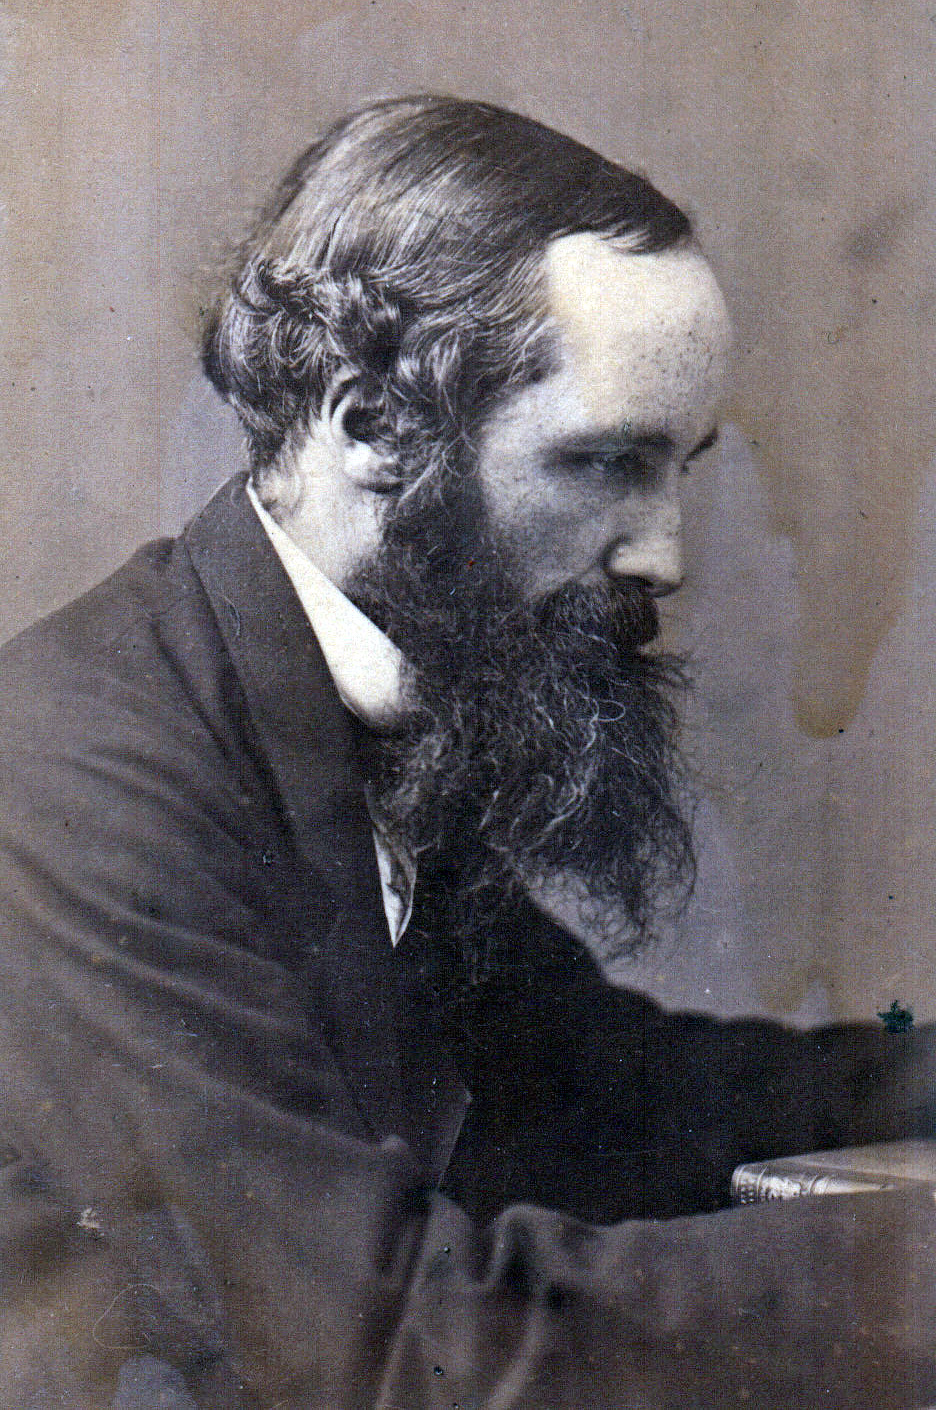
\includegraphics[width=0.3\linewidth]{images/book4/maxwell-profile.jpg}

{\small James Clerk Maxwell (1831--1879), yang menuliskan keempat persamaan bab ini lalu membaca di dalamnya keberadaan gelombang elektromagnetik yang berjalan dengan kelajuan cahaya.}
\end{omfigure}

\section{Operator vektor}

\begin{definition}[Gradien, divergensi, curl, Laplacian]\label{def:b2:maxwell-equations:operators}
\index{gradien}\index{divergensi}\index{curl}\index{Laplacian}\index{nabla}
Bagi medan skalar $f$ dan medan vektor $\vect A$, dalam koordinat
Kartesius dengan vektor lambang $\vect\nabla = (\partial_x, \partial_y,
\partial_z)$:
\begin{align*}
\operatorname{\vect{grad}}f &= \vect\nabla f = (\partial_xf,\ \partial_yf,\ \partial_zf) ,\\
\operatorname{div}\vect A &= \vect\nabla\cdot\vect A = \partial_xA_x + \partial_yA_y + \partial_zA_z ,\\
\operatorname{\vect{curl}}\vect A &= \vect\nabla\wedge\vect A = (\partial_yA_z - \partial_zA_y,\ \partial_zA_x - \partial_xA_z,\ \partial_xA_y - \partial_yA_x) ,\\
\Delta f &= \operatorname{div}\operatorname{\vect{grad}}f = \partial_x^2f + \partial_y^2f + \partial_z^2f ,
\end{align*}
dan $\Delta\vect A$ adalah Laplacian yang diambil pada tiap komponen Kartesiusnya.
Maknanya tak bergantung pada koordinat: $\operatorname{\vect{grad}}f
\cdot\dd\vect l = \dd f$ adalah perubahan $f$ sepanjang $\dd\vect l$; $\operatorname{div}
\vect A$ adalah fluks $\vect A$ yang keluar menembus permukaan sebuah volume
kecil, tiap satuan volume; $\operatorname{\vect{curl}}\vect A\cdot\vect n$ adalah
sirkulasi $\vect A$ mengelilingi simpal kecil bernormal $\vect n$, tiap satuan
luas.
\end{definition}

\begin{theorem}[Teorema divergensi dan teorema Stokes]\label{thm:b2:maxwell-equations:theorems}
\index{teorema divergensi}\index{teorema Ostrogradski}\index{teorema Stokes}
Untuk permukaan tertutup $\Sigma$ yang membatasi volume $V$, dan kurva
tertutup terorientasi $C$ yang membatasi permukaan $S$ (normalnya $\vect n$ diberikan
kaidah tangan kanan),
\[
\iint_\Sigma\vect A\cdot\vect n\,\dd S = \iiint_V\operatorname{div}\vect A\,\dd\tau ,
\qquad
\oint_C\vect A\cdot\dd\vect l = \iint_S\operatorname{\vect{curl}}\vect A\cdot\vect n\,\dd S .
\]
\end{theorem}
\admitted

\begin{remark}[Apa yang diterima tanpa bukti dan mengapa masuk akal]\label{rem:b2:maxwell-equations:whyadmitted}
Kedua teoremanya dibuktikan dalam jilid matematika Tahun ke-3;
jilid matematika tahun ini berhenti pada versi bidangnya
(Green--Riemann) dan pada integral lipat. Isinya, walau begitu, adalah
yang kita pakai dalam \cref{ch:b2:fluid-kinematics}: ubinlah volumenya dengan
kotak kecil (permukaan simpalnya dengan simpal kecil) --- fluks
menembus sisi dalamnya (sirkulasi sepanjang rusuk
dalamnya) saling meniadakan berpasangan, dan hanya batasnya yang tersisa. Dua kesamaan
menyusul dari definisinya dan dipakai terus-menerus:
$\operatorname{\vect{curl}}\operatorname{\vect{grad}}f = \vect 0$,
$\operatorname{div}\operatorname{\vect{curl}}\vect A = 0$, dan
$\operatorname{\vect{curl}}\operatorname{\vect{curl}}\vect A = \operatorname{\vect{grad}}
\operatorname{div}\vect A - \Delta\vect A$. Bagi medan yang bersimetri,
rumus yang berguna adalah: bagi medan radial $A_r(r)\vect e_r$, $\operatorname{div}
= \frac1{r^2}\partial_r(r^2A_r)$ (bola) atau $\frac1r\partial_r(rA_r)$
(tabung); bagi medan azimut $A_\theta(r)\vect e_\theta$ mengelilingi sebuah
sumbu, $(\operatorname{\vect{curl}})_z = \frac1r\partial_r(rA_\theta)$; dan bagi $f(r)$,
$\Delta f = \frac1{r^2}\partial_r(r^2\partial_rf) = \frac1r\partial_r^2(rf)$ (bola),
$\frac1r\partial_r(r\partial_rf)$ (tabung).
\end{remark}

\begin{omfigure}
\begin{tikzpicture}[font=\small, x=1cm, y=1cm, >=Stealth]
  \begin{scope}
    \draw[thick, fill=omDef!10] (0,0) rectangle (1.8,1.4);
    \draw[thick] (0,1.4) -- (0.5,1.85) -- (2.3,1.85) -- (1.8,1.4);
    \draw[thick] (1.8,0) -- (2.3,0.45) -- (2.3,1.85);
    \draw[omThm, thick, ->] (-0.9,0.7) -- (-0.1,0.7);
    \draw[omThm, thick, ->] (1.9,0.7) -- (3.0,0.7);
    \draw[omThm, thick, ->] (0.9,-0.8) -- (0.9,-0.1);
    \draw[omThm, thick, ->] (1.1,1.9) -- (1.1,2.7);
    \node[font=\footnotesize] at (1.0,-1.35) {$\operatorname{div}\vect A = \dfrac{\text{fluks yang keluar}}{\text{volume}}$};
  \end{scope}
  \begin{scope}[xshift=7.6cm]
    \draw[thick, omDef, postaction={decorate, decoration={markings, mark=at position 0.15 with {\arrow{>}}, mark=at position 0.65 with {\arrow{>}}}}] (-1.2,0) rectangle (1.2,1.4);
    \draw[omExo, thick, ->] (0,0.7) -- (0,2.3) node[right, font=\footnotesize] {$\vect n$};
    \foreach \x in {-0.8,0,0.8} \draw[omThm, ->] ({\x-0.3},1.05) -- ({\x+0.3},1.05);
    \foreach \x in {-0.8,0,0.8} \draw[omThm, ->] ({\x+0.15},0.35) -- ({\x-0.15},0.35);
    \node[font=\footnotesize] at (0,-0.8) {$\operatorname{\vect{curl}}\vect A\cdot\vect n = \dfrac{\text{sirkulasi}}{\text{luas}}$};
  \end{scope}
\end{tikzpicture}

{\small Kedua operator \omterm{thm:b2:maxwell-equations:maxwell}{persamaan Maxwell}, yang dibaca
secara geometris: \omterm{def:b2:maxwell-equations:operators}{divergensi} mengukur seberapa banyak sebuah medan mengalir keluar dari
volume kecil, \omterm{def:b2:maxwell-equations:operators}{curl} seberapa banyak ia bersirkulasi mengelilingi simpal kecil.}
\end{omfigure}

\section{Keempat persamaannya}

\begin{theorem}[Persamaan Maxwell]\label{thm:b2:maxwell-equations:maxwell}
\index{persamaan Maxwell}\index{persamaan Maxwell--Gauss}\index{persamaan Maxwell--Faraday}\index{persamaan Maxwell--Ampère}\index{arus pergeseran}
Dalam hampa (dan dalam materi yang dilukiskan \omterm{def:b2:charges-currents-conduction:densities}{rapat muatan} dan \omterm{def:b2:charges-currents-conduction:densities}{rapat
arus} totalnya $\rho$ dan $\vect j$), medan listrik dan medan magnetnya menuruti, di
setiap titik dan setiap waktu,
\begin{align*}
\operatorname{div}\vect E &= \frac\rho{\varepsilon_0} &&\text{(Maxwell--Gauss)} , &
\operatorname{\vect{curl}}\vect E &= -\frac{\partial\vect B}{\partial t} &&\text{(Maxwell--Faraday)} ,\\
\operatorname{div}\vect B &= 0 &&\text{(Maxwell--flux)} , &
\operatorname{\vect{curl}}\vect B &= \mu_0\vect j + \mu_0\varepsilon_0\frac{\partial\vect E}{\partial t} &&\text{(Maxwell--Ampère)} ,
\end{align*}
dengan $\varepsilon_0 = \qty{8.85e-12}{F/m}$, $\mu_0 = 4\pi \times \qty{1e-7}{H/m}$ (dan
$\varepsilon_0\mu_0 = 1/c^2$). Medannya bekerja pada muatan lewat gaya
Lorentz $\vect F = q(\vect E + \vect v\wedge\vect B)$. Suku $\varepsilon_0\partial_t\vect E$
adalah rapat \emph{\omterm{thm:b2:maxwell-equations:maxwell}{arus pergeseran}} Maxwell.
\end{theorem}

\begin{proof}[Kesetaraan dengan hukum integral jilid Tahun ke-1]
Terapkanlah teorema \omterm{def:b2:maxwell-equations:operators}{divergensi} pada kedua yang pertama: $\iint_\Sigma\vect E\cdot
\vect n\,\dd S = Q_{\text{dlm}}/\varepsilon_0$ (Gauss) dan fluks $\vect B$
menembus permukaan tertutup mana pun bernilai nol. Terapkanlah Stokes pada kedua yang terakhir:
$\oint_C\vect E\cdot\dd\vect l = -\dd\Phi_B/\dd t$ (Faraday, bagi simpal tetap)
dan $\oint_C\vect B\cdot\dd\vect l = \mu_0I_{\text{lingkup}} + \mu_0\varepsilon_0\,\dd\Phi_E/\dd t$
(Ampère, yang telah dilengkapi). Sebaliknya hukum integralnya, yang berlaku bagi setiap
volume dan simpal, menyiratkan hukum lokalnya. Persamaan lokalnya karena itu
adalah hukum Tahun ke-1 ditambah satu suku baru, yang dibenarkan di bawah; keduanya diambil sebagai
postulat elektromagnetisme.
\end{proof}

\begin{proposition}[Mengapa arus pergeserannya diperlukan]\label{prop:b2:maxwell-equations:displacement}
Mengambil \omterm{def:b2:maxwell-equations:operators}{divergensi} \omterm{thm:b2:maxwell-equations:maxwell}{persamaan Maxwell--Ampère} lalu memakai
$\operatorname{div}\operatorname{\vect{curl}} = 0$ dan Maxwell--Gauss memberi
\[
0 = \mu_0\operatorname{div}\vect j + \mu_0\varepsilon_0\,\partial_t\operatorname{div}\vect E
= \mu_0\Bigl(\operatorname{div}\vect j + \frac{\partial\rho}{\partial t}\Bigr) :
\]
persamaannya memuat kekekalan muatan. Tanpa suku
pergeserannya persamaan itu akan menuntut $\operatorname{div}\vect j = 0$ selalu
--- keliru dalam kapasitor yang sedang diisi, tempat arus hantarannya berhenti
di kepingnya. Di sana, di antara kepingnya, $\varepsilon_0\partial_t\vect E$ mengemban
tepat arus yang tiba dalam kawatnya, dan medan magnetnya
bersirkulasi mengelilingi celahnya seperti mengelilingi sebuah kawat.
\end{proposition}

\begin{proof}
\omterm{def:b2:maxwell-equations:operators}{Divergensi} kedua ruasnya, seperti dinyatakan; bagi kapasitornya, fluks
$\varepsilon_0\partial_t\vect E$ menembus sebuah permukaan di antara kepingnya adalah
$\varepsilon_0S\,\dd E/\dd t = \dd Q/\dd t = I$.
\end{proof}

\begin{example}[Medan di dalam kapasitor yang sedang diisi]\label{ex:b2:maxwell-equations:capacitor}
Keping lingkaran berjari-jari $R$, berjarak $d \ll R$, diisi arus
$I$: di antaranya $E = Q/\varepsilon_0\pi R^2$ seragam dan tumbuh dengan $\dd E/
\dd t = I/\varepsilon_0\pi R^2$. Menurut simetrinya $\vect B = B(r)\vect e_\theta$; Ampère--Maxwell
pada lingkaran berjari-jari $r < R$ (tak ada arus hantaran yang menyeberanginya): $2\pi rB
= \mu_0\varepsilon_0\pi r^2\,\dd E/\dd t$, jadi $B = \mu_0Ir/2\pi R^2$ --- yaitu medan
arus seragam $I$ yang tersebar pada cakramnya, sinambung di $r = R$ dengan
$\mu_0I/2\pi r$ kawatnya di luar. Untuk $I = \qty{1}{A}$, $R = \qty{5}{cm}$: $B(R) =
\qty{4}{\micro T}$, terukurkan; suku Maxwell itu nyata.
\end{example}

\begin{omfigure}
\begin{tikzpicture}[font=\small, x=1cm, y=1cm, >=Stealth]
  \draw[thick, omThm] (-4.0,0) -- (-1.3,0); \draw[thick, omThm] (1.3,0) -- (4.0,0);
  \draw[omThm, very thick, ->] (-3.4,0.25) -- (-2.4,0.25) node[above, font=\footnotesize, pos=0.5] {$I$};
  \draw[omThm, very thick, ->] (2.4,0.25) -- (3.4,0.25) node[above, font=\footnotesize, pos=0.5] {$I$};
  \draw[thick, fill=omExo!40] (-1.3,-1.4) rectangle (-1.1,1.4);
  \draw[thick, fill=omExo!40] (1.1,-1.4) rectangle (1.3,1.4);
  \foreach \y in {-1.0,-0.5,0,0.5,1.0} \draw[omDef, ->] (-1.05,\y) -- (1.05,\y);
  \node[omDef, font=\footnotesize] at (0,1.25) {$\vect E(t)$};
  \draw[omProp, thick] (0,0) ellipse (0.5 and 1.7);
  \draw[omProp, thick, ->] (0.5,0.05) -- (0.5,-0.05);
  \node[omProp, font=\footnotesize] at (0.95,-1.75) {$\vect B$};
  \node[font=\footnotesize] at (0,-2.3) {$\oint\vect B\cdot\dd\vect l = \mu_0\varepsilon_0\,\dfrac{\dd\Phi_E}{\dd t} = \mu_0 I$};
\end{tikzpicture}

{\small Sebuah kapasitor yang sedang diisi: tak ada muatan yang menyeberangi celahnya, tetapi
fluks listrik menembus sebuah simpal di sekelilingnya tumbuh; suku Maxwell memberi
simpalnya sirkulasi $\vect B$ yang sama seolah-olah kawatnya berlanjut ---
yaitu \omterm{thm:b2:maxwell-equations:maxwell}{arus pergeseran}.}
\end{omfigure}

\begin{remark}[Kelinearan; apa yang dikatakan persamaannya]\label{rem:b2:maxwell-equations:linearity}
Persamaannya linear dalam medannya dan sumbernya: medannya
bertumpang. Dua di antaranya (Gauss, Faraday--fluks) tak mengemban sumber dan
menyatakan struktur --- garis medan listrik bermula dan berakhir pada muatan,
garis medan magnet tak pernah berakhir; kedua yang lain mengatakan bagaimana muatan dan
arus, serta perubahan tiap medannya, menciptakan medannya. Dibaca
bersama-sama, $\vect B$ yang berubah membuat $\vect E$ bersirkulasi dan $\vect E$ yang
berubah membuat $\vect B$ bersirkulasi: keduanya dapat saling melangsungkan tanpa
muatan di mana pun --- itulah gelombang
\cref{ch:b2:plane-waves-polarization}, dan arus pergeserannyalah yang
membuatnya mungkin.
\end{remark}

\section{Potensial}

\begin{proposition}[Potensial skalar dan potensial vektor]\label{prop:b2:maxwell-equations:potentials}
\index{potensial vektor}\index{potensial skalar}\index{tera}
\index{tera Coulomb}\index{persamaan Poisson}
Karena $\operatorname{div}\vect B = 0$ dan $\operatorname{\vect{curl}}\vect E = -\partial_t
\vect B$, medannya diturunkan dari sebuah \emph{\omterm{prop:b2:maxwell-equations:potentials}{potensial vektor}} $\vect A$ dan sebuah
\emph{\omterm{prop:b2:maxwell-equations:potentials}{potensial skalar}} $V$:
\[
\vect B = \operatorname{\vect{curl}}\vect A , \qquad
\vect E = -\operatorname{\vect{grad}}V - \frac{\partial\vect A}{\partial t} ,
\]
yang tertentukan sampai sebuah \emph{transformasi tera} $\vect A \to \vect A +
\operatorname{\vect{grad}}\chi$, $V \to V - \partial_t\chi$, yang membiarkan medannya
tak berubah. Dalam \emph{\omterm{prop:b2:maxwell-equations:potentials}{tera Coulomb}} $\operatorname{div}\vect A = 0$, hukum
Gauss menjadi \emph{\omterm{prop:b2:maxwell-equations:potentials}{persamaan Poisson}}
\[
\Delta V = -\frac\rho{\varepsilon_0} ,
\]
dan dalam rezim tunak hukum Ampère menjadi $\Delta\vect A = -\mu_0\vect j$.
Dalam statika $V$ adalah potensial elektrostatik jilid Tahun ke-1.
\end{proposition}

\begin{proof}
Medan yang bebas \omterm{def:b2:maxwell-equations:operators}{divergensi} adalah sebuah \omterm{def:b2:maxwell-equations:operators}{curl} (diterima tanpa bukti, seperti pernyataan
kebalikannya bahwa medan yang bebas \omterm{def:b2:maxwell-equations:operators}{curl} adalah sebuah \omterm{def:b2:maxwell-equations:operators}{gradien}, keduanya dari jilid
matematika Tahun ke-2 bagi daerah terhubung sederhana); lalu $\operatorname{\vect{curl}}
(\vect E + \partial_t\vect A) = \vect 0$, jadi $\vect E + \partial_t\vect A$ adalah sebuah \omterm{def:b2:maxwell-equations:operators}{gradien}.
Teranya: $\operatorname{\vect{curl}}\operatorname{\vect{grad}}\chi = \vect 0$ dan
suku $\partial_t\operatorname{\vect{grad}}\chi$-nya saling meniadakan dalam $\vect E$. Poisson: $\operatorname{div}
\vect E = -\Delta V - \partial_t\operatorname{div}\vect A$. Statika: $\operatorname{\vect{curl}}
\operatorname{\vect{curl}}\vect A = \operatorname{\vect{grad}}\operatorname{div}\vect A - \Delta\vect A
= \mu_0\vect j$.
\end{proof}

\begin{example}[Dua potensial vektor]\label{ex:b2:maxwell-equations:vectorpot}
Medan seragam $\vect B_0$ diturunkan dari $\vect A = \tfrac12\vect B_0\wedge\vect r$
(periksalah: $\operatorname{\vect{curl}}(\tfrac12\vect B_0\wedge\vect r) = \vect B_0$, dan
$\operatorname{div}\vect A = 0$); di dalam solenoida tak hingga ini menjadi $A_\theta =
Br/2$, di luarnya $A_\theta = BR^2/2r$ --- sebuah potensial yang tidak lenyap
di tempat medannya lenyap, dan yang sirkulasinya sepanjang sebuah simpal adalah fluks
$\vect B$ menembusnya: $\oint\vect A\cdot\dd\vect l = \Phi_B$ (Stokes). Hukum Faraday
lalu berbunyi $\vect E = -\partial_t\vect A$ bagi medan imbasnya.
\end{example}

\section{Medan di sebuah antarmuka}

\begin{proposition}[Hubungan batas]\label{prop:b2:maxwell-equations:boundary}
\index{hubungan batas (medan)}\index{arus permukaan}
Menyeberangi permukaan yang mengemban \omterm{def:b2:charges-currents-conduction:densities}{rapat muatan} permukaan $\sigma$ dan
rapat \omterm{prop:b2:maxwell-equations:boundary}{arus permukaan} $\vect j_s$ (\unit{A/m}), dengan $\vect n_{12}$ yaitu
normal satuan dari medium 1 ke medium 2,
\[
\vect E_2 - \vect E_1 = \frac\sigma{\varepsilon_0}\,\vect n_{12} , \qquad
\vect B_2 - \vect B_1 = \mu_0\,\vect j_s\wedge\vect n_{12} :
\]
komponen tangensial $\vect E$ dan komponen normal $\vect B$
sinambung; komponen normal $\vect E$ melompat sebesar $\sigma/\varepsilon_0$,
komponen tangensial $\vect B$ sebesar $\mu_0j_s$. Di permukaan sebuah
penghantar sempurna ($\vect E = \vect B = \vect 0$ di dalamnya, dalam hal-hal
\cref{ch:b2:wave-interfaces}), $\vect E$ bersifat normal dan sama dengan $\sigma\vect n/
\varepsilon_0$, $\vect B$ bersifat tangensial dan sama dengan $\mu_0\vect j_s\wedge\vect n$.
\end{proposition}

\begin{proof}
Komponen normalnya: hukum Gauss dan hukum fluks pada kotak pipih datar
yang mengangkangi permukaannya, seluas $\dd S$ dan bertinggi lenyap: $(E_{2n}
- E_{1n})\dd S = \sigma\dd S/\varepsilon_0$, $(B_{2n} - B_{1n})\dd S = 0$. Komponen
tangensialnya: hukum Faraday dan hukum Ampère pada persegi panjang kecil
yang mengangkangi permukaannya, sepanjang $\dd l$ dan bertinggi lenyap:
fluks $\partial_t\vect B$ dan $\partial_t\vect E$ menembus persegi panjangnya lenyap
bersama luasnya, tetapi sebuah \omterm{prop:b2:maxwell-equations:boundary}{arus permukaan} $j_s\,\dd l$ menyeberanginya:
$(E_{2t} - E_{1t})\dd l = 0$, $(B_{2t} - B_{1t})\dd l = \mu_0j_s\dd l$ bagi
arah tangensial yang tegak lurus $\vect j_s$.
\end{proof}

\begin{omfigure}
\begin{tikzpicture}[font=\small, x=1cm, y=1cm, >=Stealth]
  \begin{scope}
    \fill[omExo!15] (-2.6,-1.3) rectangle (2.6,0); \draw[thick] (-2.6,0) -- (2.6,0);
    \node[font=\footnotesize] at (-2.2,0.4) {medium 2}; \node[font=\footnotesize] at (-2.2,-0.4) {medium 1};
    \node[omThm, font=\footnotesize] at (1.8,0.25) {$\sigma$, $\vect j_s$};
    \draw[omDef, thick] (0,0.35) ellipse (0.7 and 0.18); \draw[omDef, thick] (0,-0.35) ellipse (0.7 and 0.18);
    \draw[omDef, thick] (-0.7,0.35) -- (-0.7,-0.35) (0.7,0.35) -- (0.7,-0.35);
    \draw[omDef, thick, ->] (0,0.35) -- (0,1.1) node[right, font=\footnotesize] {$\vect n_{12}$};
    \node[font=\footnotesize] at (0,-1.7) {kotak pipih: $E_{2n} - E_{1n} = \sigma/\varepsilon_0$, $B_{2n} = B_{1n}$};
  \end{scope}
  \begin{scope}[xshift=7.4cm]
    \fill[omExo!15] (-2.6,-1.3) rectangle (2.6,0); \draw[thick] (-2.6,0) -- (2.6,0);
    \draw[omProp, thick, postaction={decorate, decoration={markings, mark=at position 0.3 with {\arrow{>}}, mark=at position 0.8 with {\arrow{>}}}}] (-1.0,-0.3) rectangle (1.0,0.3);
    \node[omProp, font=\footnotesize] at (0,0.6) {$\dd l$};
    \node[omThm, font=\footnotesize] at (1.9,-0.25) {$\vect j_s$ (masuk halaman)};
    \foreach \x in {-1.6,-0.8,0,0.8,1.6} \node[omThm, font=\scriptsize] at (\x,-0.02) {$\otimes$};
    \node[font=\footnotesize] at (0,-1.7) {simpal: $E_{2t} = E_{1t}$, $B_{2t} - B_{1t} = \mu_0j_s$};
  \end{scope}
\end{tikzpicture}

{\small Hubungan batasnya datang dari hukum integral yang diterapkan pada
sebuah kotak pipih datar dan sebuah simpal tipis yang mengangkangi antarmukanya: muatan
permukaan membuat $\vect E$ normalnya melompat, \omterm{prop:b2:maxwell-equations:boundary}{arus permukaan} membuat
$\vect B$ tangensialnya melompat; komponen lainnya sinambung.}
\end{omfigure}

\begin{example}[Bidang bermuatan, lembar arus, solenoida]\label{ex:b2:maxwell-equations:sheets}
Sebuah bidang dengan $\sigma$ sendirian dalam ruang: menurut simetrinya $\vect E = \pm E\vect n$ pada
kedua sisinya, dan lompatannya $2E = \sigma/\varepsilon_0$ memberi $E = \sigma/2\varepsilon_0$ ---
hasil Tahun ke-1 dalam satu baris. Sebuah lembar arus bidang $j_s$: $B =
\mu_0j_s/2$ pada tiap sisinya, berlawanan arah. Sebuah solenoida panjang berlilitan $n$ tiap
meter yang mengemban $I$ adalah lembar arus tabung $j_s = nI$: lompatannya
$\mu_0nI$ menyeberanginya, dengan $B = 0$ di luar, memberi $B = \mu_0nI$ di dalam.
\end{example}

\section{Rezim kuasi-tunak}

\begin{definition}[Hampiran kuasi-tunak]\label{def:b2:maxwell-equations:arqs}
\index{hampiran kuasi-tunak}\index{ARQS}
Sebuah sistem berukuran $L$ yang digerakkan pada frekuensi $f$ bersifat \emph{kuasi-tunak}
apabila $L \ll \lambda = c/f$: waktu $L/c$ yang diperlukan medannya untuk menyeberanginya
dapat diabaikan dibandingkan periodenya, dan semua titiknya ``melihat''
sumbernya pada saat yang sama. Dua limitnya dipakai:
\begin{itemize}
  \item rezim kuasi-tunak \emph{magnetik} (rangkaian dengan
        arus, kumparan, transformator, imbasan): \omterm{thm:b2:maxwell-equations:maxwell}{arus pergeserannya}
        dibuang dari hukum Ampère, $\operatorname{\vect{curl}}\vect B
        = \mu_0\vect j$ (sehingga $\operatorname{div}\vect j = 0$ dan arusnya mengalir dalam
        rangkaian tertutup), sementara hukum Faraday disimpan seutuhnya;
  \item rezim kuasi-tunak \emph{listrik} (sebuah kapasitor yang
        sedang diisi): suku Faradaynya dibuang, $\vect E$ adalah
        medan elektrostatik muatan seketikanya, sementara
        \omterm{thm:b2:maxwell-equations:maxwell}{arus pergeserannya} disimpan untuk mencari $\vect B$.
\end{itemize}
\end{definition}

\begin{proof}[Pembenaran]
Dalam rezim magnetiknya, bandingkanlah kedua suku hukum Ampère dalam sebuah
penghantar: $\mu_0\varepsilon_0\partial_t E \sim \mu_0\varepsilon_0\omega E$ melawan $\mu_0\gamma E$,
dengan nisbah $\varepsilon_0\omega/\gamma = \omega\tau_r \sim 10^{-17}$ pada \qty{50}{Hz} dalam tembaga;
di luar penghantarnya \omterm{thm:b2:maxwell-equations:maxwell}{arus pergeserannya} berorde
$\varepsilon_0\omega E$ dengan $E \sim \omega AB$, yakni lebih kecil daripada pengaruh arus
hantarannya sebesar $(\omega L/c)^2 = (L/\lambda)^2 \times 4\pi^2$. Dalam rezim
listriknya medan imbasnya $\omega BL \sim \omega^2\varepsilon_0\mu_0L^2E$ lebih kecil daripada $E$
sebesar $(L/\lambda)^2$ yang sama.
\end{proof}

\begin{example}[Rangkaian dan antena]\label{ex:b2:maxwell-equations:sizes}
Sebuah rangkaian jala-jala pada \qty{50}{Hz} ($\lambda = \qty{6000}{km}$) bersifat kuasi-tunak
sampai ukuran sebuah negara --- itulah sebabnya hukum Kirchhoff dan
transformator bekerja. Rangkaian \qty{10}{cm} bersifat kuasi-tunak sampai sekitar
\qty{100}{MHz}; pada \qty{1}{GHz} ($\lambda = \qty{30}{cm}$) kawatnya menjadi antena,
arusnya berbeda-beda sepanjang sebuah kawat, dan rangkaiannya memancar: yaitu ranah
\cref{ch:b2:dipole-radiation} dan ranah rancangan gelombang mikro, tempat sebuah jalur pada
papan menjadi sebuah \omterm{prop:b2:dispersion-wave-packets:coax}{saluran transmisi}.
\end{example}

\begin{omfigure}
\begin{tikzpicture}
\begin{axis}[omaxis, axis x line=bottom, axis y line=left, width=8.6cm, height=5.0cm,
    xmode=log, ymode=log, xmin=1, xmax=1e10, ymin=3e-4, ymax=1e4,
    xlabel={$f$ (Hz)}, ylabel={$L$ (m)}, xtick={1,1e2,1e4,1e6,1e8,1e10}, ytick={1e-3,1,1e3},
    xlabel style={at={(axis description cs:0.5,-0.12)}, anchor=north},
    ylabel style={at={(axis description cs:-0.1,0.5)}, rotate=90, anchor=south}, samples=50]
  \addplot[omThm, thick, domain=1:1e10] {3e8/x};
  \addplot[omThm, dashed, domain=1:1e10] {3e7/x};
  \node[font=\scriptsize, anchor=west] at (axis cs:1e6,4e3) {$L \gtrsim \lambda$: gelombang, pemancaran};
  \node[font=\scriptsize, anchor=west] at (axis cs:10,3e-2) {$L \ll \lambda$: kuasi-tunak, rangkaian};
  \node[font=\scriptsize, omDef] at (axis cs:50,1) {jala-jala};
  \node[font=\scriptsize, omDef, anchor=east] at (axis cs:3e7,0.1) {telepon seluler};
  \node[font=\scriptsize, omDef, anchor=east] at (axis cs:3e9,1e-3) {cip};
\end{axis}
\end{tikzpicture}

{\small Ukuran terhadap frekuensi: di bawah garis $L = \lambda/10$ (putus-putus) sebuah
perangkat bersifat kuasi-tunak dan hukum rangkaiannya berlaku; dekat dan di atas
$L = \lambda$ medannya merambat, dan perangkatnya memancar.}
\end{omfigure}

\begin{method}[Memakai persamaan lokalnya]\label{met:b2:maxwell-equations:method}
(1) Pakailah simetri dan ketakubahan sumbernya untuk menetapkan
arah dan variabel medannya (seperti dalam jilid Tahun ke-1).
(2) Pilihlah bentuknya: integral (Gauss, Ampère pada permukaan atau simpal
yang dipilih baik-baik) ketika simetrinya cukup; lokal ketika Anda memerlukan
persamaan diferensial (Poisson bagi $V$, persamaan difusi atau \omterm{thm:b2:waves-on-strings:equation}{persamaan gelombang}
bagi medannya). (3) Dalam soal yang bergantung waktu putuskanlah rezimnya:
statik, kuasi-tunak magnetik atau listrik, atau Maxwell penuh. (4)
Di antarmuka, pakailah hubungan batasnya --- di situlah satu-satunya tempat
muatan dan \omterm{prop:b2:maxwell-equations:boundary}{arus permukaan} masuk. (5) Periksalah
$\operatorname{div}\vect B = 0$ dan dimensinya.
\end{method}

\section{Latihan}

\begin{exercise}[$\star$]\label{exo:b2:maxwell-equations:1}
Hitunglah \omterm{def:b2:maxwell-equations:operators}{divergensi} dan \omterm{def:b2:maxwell-equations:operators}{curl} (a) $\vect A = (x, y, z)$; (b)
$\vect A = (-y, x, 0)$; (c) $\vect A = (yz, zx, xy)$; (d) $\vect A = \vect r/r^3$
(pakailah rumus radialnya, $r \ne 0$); (e) $\vect A = (0, 0, x^2)$. Mana yang berupa
\omterm{def:b2:maxwell-equations:operators}{gradien}, mana yang berupa \omterm{def:b2:maxwell-equations:operators}{curl}, mana yang bukan keduanya?
\end{exercise}

\begin{exercise}[$\star$]\label{exo:b2:maxwell-equations:2}
(a) Periksalah dimensi tiap suku keempat \omterm{thm:b2:maxwell-equations:maxwell}{persamaan Maxwell}.
(b) Hitunglah $1/\sqrt{\varepsilon_0\mu_0}$. (c) Nisbah rapat \omterm{thm:b2:maxwell-equations:maxwell}{arus pergeseran}
terhadap \omterm{def:b2:charges-currents-conduction:densities}{rapat arus} hantaran dalam tembaga pada \qty{50}{Hz}, dalam
air laut ($\gamma = \qty{5}{S/m}$) pada \qty{1}{GHz}, dalam kaca ($\gamma =
\qty{1e-12}{S/m}$, $\varepsilon_0$ diambil demi kesederhanaan) pada \qty{50}{Hz}: mana yang
``penghantar'' bagi masing-masingnya?
\end{exercise}

\begin{exercise}[$\star$]\label{exo:b2:maxwell-equations:3}
Sebuah kapasitor berkeping lingkaran ($R = \qty{10}{cm}$, $d = \qty{2}{mm}$)
diisi $I = \qty{0.5}{A}$. Tentukanlah laju perubahan $E$; rapat \omterm{thm:b2:maxwell-equations:maxwell}{arus
pergeserannya}; $B$ pada $r = \qty{5}{cm}$ dan pada $r = \qty{20}{cm}$ (dalam
bidang di tengah-tengah kepingnya); bandingkanlah yang terakhir dengan medan
kawat penyuapnya pada jarak yang sama.
\end{exercise}

\begin{exercise}[$\star$]\label{exo:b2:maxwell-equations:4}
(a) $\vect E = kx\,\vect e_x$ mengisi sebuah daerah: \omterm{def:b2:charges-currents-conduction:densities}{rapat muatan} di sana. (b)
Di dalam sebuah bola berjari-jari $R$, $\vect E = (\rho_0r/3\varepsilon_0)\vect e_r$: periksalah dengan
\omterm{def:b2:maxwell-equations:operators}{divergensi} radialnya bahwa $\rho = \rho_0$, lalu dapatkanlah kembali medan di luarnya
dari hukum integral Gauss. (c) $\vect B = B_0(y/a)\vect e_x$: mungkinkah ia sebuah
medan magnet? \omterm{def:b2:charges-currents-conduction:densities}{Rapat arus} apa yang melangsungkannya?
\end{exercise}

\begin{exercise}[$\star\star$]\label{exo:b2:maxwell-equations:5}
\emph{\omterm{prop:b2:maxwell-equations:potentials}{Potensial vektor}.} (a) Tunjukkanlah bahwa $\vect A = \tfrac12\vect B_0\wedge\vect r$
memberi $\operatorname{\vect{curl}}\vect A = \vect B_0$ dan $\operatorname{div}\vect A = 0$.
(b) Demikian pula $\vect A' = B_0x\,\vect e_y$: carilah fungsi tera $\chi$ dengan
$\vect A' = \vect A + \operatorname{\vect{grad}}\chi$. (c) Solenoida berjari-jari $R$,
bermedan $B$ di dalamnya: periksalah $A_\theta = Br/2$ ($r < R$) dan $BR^2/2r$ ($r > R$)
dengan $(\operatorname{\vect{curl}}\vect A)_z = \frac1r\partial_r(rA_\theta)$; kesinambungannya di $R$.
(d) Sirkulasi $\vect A$ pada lingkaran berjari-jari $r > R$ dan fluks
$\vect B$: apa katanya tentang ggl imbas dalam sebuah simpal di luar sebuah
solenoida yang arusnya berubah-ubah?
\end{exercise}

\begin{exercise}[$\star\star$]\label{exo:b2:maxwell-equations:6}
\emph{Hubungan batas.} (a) Sebuah penghantar dalam kesetimbangan
elektrostatik mengemban $\sigma$ pada permukaannya: medan tepat di luarnya (dari
lompatannya, dengan $\vect E = \vect 0$ di dalamnya); untuk $\sigma = \qty{1}{\micro C/m^2}$. (b) Dua
bidang sejajar dengan $+\sigma$ dan $-\sigma$: medannya di mana-mana, lewat lompatannya.
(c) Sebuah solenoida panjang ($n = \qty{2000}{m^{-1}}$, $I = \qty{5}{A}$) sebagai lembar
arus: $j_s$, lompatan $B$, dan $B$ di dalamnya. (d) Sebuah kumparan toroida: mengapa $B$
nol di luar dan $\mu_0NI/2\pi r$ di dalam, dari lompatan yang sama?
\end{exercise}

\begin{exercise}[$\star\star$]\label{exo:b2:maxwell-equations:7}
\emph{Poisson dalam satu dimensi.} Antara dua elektrode bidang di $x = 0$
($V = 0$) dan $x = d$ ($V = U$), sebuah \omterm{def:b2:charges-currents-conduction:densities}{rapat muatan} seragam $\rho_0$ mengisi
celahnya (sebuah muatan ruang). (a) Selesaikanlah \omterm{prop:b2:maxwell-equations:potentials}{persamaan Poisson} bagi $V(x)$. (b) Medannya
$E(x)$; di manakah ia nol jika $\rho_0 > 0$ dan besar? (c) Muatan permukaan pada
kedua elektrodenya, dari hubungan batasnya. (d) Dengan $\rho_0 = 0$
dapatkanlah kembali kapasitornya; dengan $U = 0$, sketsalah $V$.
\end{exercise}

\begin{exercise}[$\star\star$]\label{exo:b2:maxwell-equations:8}
\emph{Kuasi-tunak atau tidak.} (a) $\lambda$ pada \qty{50}{Hz}, \qty{1}{MHz},
\qty{100}{MHz}, \qty{2.4}{GHz}. (b) Sampai frekuensi berapa rangkaian \qty{10}{cm}
bersifat kuasi-tunak (kriteria $L < \lambda/10$)? Sebuah cip \qty{1}{cm}? Sebuah
jaringan daya \qty{1000}{km}? (c) Dalam kapasitor berjari-jari $R = \qty{5}{cm}$ pada
\qty{1}{MHz}, perkirakanlah nisbah medan listrik imbasnya (dari
$\vect B$ yang berubah pada latihan sebelumnya) terhadap medan utamanya: $(\omega R/c)^2
/4$. (d) Mengapa frekuensi jala-jala sebuah jaringan selebar benua merupakan soal
kuasi-tunak walaupun jaringannya selebar \qty{1000}{km}?
\end{exercise}

\begin{exercise}[$\star\star$]\label{exo:b2:maxwell-equations:9}
Tunjukkanlah bahwa hukum Ampère tanpa \omterm{thm:b2:maxwell-equations:maxwell}{arus pergeseran}, $\operatorname{\vect{curl}}
\vect B = \mu_0\vect j$, berlawanan dengan kekekalan muatan setiap kali $\partial_t\rho
\ne 0$. Dalam kapasitor \cref{exo:b2:maxwell-equations:3}, taksirlah
$\operatorname{div}\vect j$ yang dirata-ratakan atas sebuah keping setebal $e = \qty{0.1}{mm}$
(tempat arus $I$ berhenti), dan $\partial_t\rho$ yang bersesuaian.
\end{exercise}

\begin{exercise}[$\star\star\star$]\label{exo:b2:maxwell-equations:10}
\emph{Betatron.} Sebuah medan magnet seragam $B(t)\vect e_z$ mengisi
sebuah tabung berjari-jari $R$, yang tumbuh dengan $\dd B/\dd t = \dot B$. (a) Menurut simetrinya
$\vect E = E_\theta(r)\vect e_\theta$: pakailah hukum Faraday integral untuk mencari $E_\theta$
bagi $r < R$ dan $r > R$. (b) Tak ada muatan di mana pun: berilah tanggapan atas sebuah
medan listrik yang garisnya tertutup. (c) Sebuah elektron pada lingkaran berjari-jari
$r_0 < R$ memperoleh berapa energi tiap putaran? Untuk $\dot B = \qty{10}{T/s}$,
$r_0 = \qty{0.5}{m}$: energinya tiap putaran dalam eV; jumlah putaran yang diperlukan bagi \qty{20}{MeV}.
(d) Agar jari-jari orbitnya tetap, momentumnya $p = eBr_0$ (dari
gaya magnetiknya) harus tumbuh sebagaimana dituntut energi yang diperoleh dari medan imbasnya:
tunjukkanlah syaratnya $B(r_0) = \tfrac12\langle B\rangle_{\text{cakram}}$
--- yaitu syarat betatron.
\end{exercise}

\begin{exercise}[$\star\star\star$]\label{exo:b2:maxwell-equations:11}
\emph{Gelombang Maxwell.} Dalam hampa ($\rho = 0$, $\vect j = \vect 0$): (a) ambillah
\omterm{def:b2:maxwell-equations:operators}{curl} \omterm{thm:b2:maxwell-equations:maxwell}{persamaan Maxwell--Faraday}, pakailah $\operatorname{\vect{curl}}
\operatorname{\vect{curl}} = \operatorname{\vect{grad}}\operatorname{div} - \Delta$ dan persamaan
lainnya untuk memperoleh $\Delta\vect E = \mu_0\varepsilon_0\,\partial_t^2\vect E$. (b) Hal yang sama bagi
$\vect B$. (c) Ini adalah \omterm{thm:b2:waves-on-strings:equation}{persamaan d'Alembert} dalam tiga dimensi: kelajuannya?
Hitunglah dari $\varepsilon_0$ dan $\mu_0$. (d) Mengapa bilangan ini meyakinkan
Maxwell bahwa cahaya bersifat elektromagnetik, dan pengukuran
Weber serta Kohlrausch yang mana yang dipakainya?
\end{exercise}

\begin{exercise}[$\star\star\star$]\label{exo:b2:maxwell-equations:12}
\emph{Medan dalam penghantar pada frekuensi rendah.} Dalam penghantar ohmik
($\vect j = \gamma\vect E$) dalam rezim kuasi-tunak magnetik: (a) ambillah
\omterm{def:b2:maxwell-equations:operators}{curl} hukum Ampère lalu pakailah hukum Faraday untuk menunjukkan $\Delta\vect B = \mu_0\gamma\,
\partial_t\vect B$; mengapa ia sebuah persamaan difusi? (b) Waktu ciri
bagi $\vect B$ untuk menembus kedalaman $d$: $\tau \sim \mu_0\gamma d^2$; angkanya bagi
keping tembaga \qty{1}{cm} dan bagi inti Bumi ($\gamma \approx \qty{5e5}{S/m}$,
$d \approx \qty{3000}{km}$). (c) Pada frekuensi $f$, kedalaman yang tercapai dalam satu
periode: tunjukkanlah ia berorde $\delta = \sqrt{2/\mu_0\gamma\omega}$; nilainya bagi tembaga
pada \qty{50}{Hz} dan \qty{1}{MHz} (yaitu \omterm{def:b2:dispersion-wave-packets:complex}{kedalaman kulit}
\cref{ch:b2:waves-in-media}). (d) Apa sirat (b) bagi perubahan
menurut waktu medan magnet Bumi?
\end{exercise}

\section{Soal: Kapasitor, betatron dan potensialnya}

\begin{problem}[{Soal akhir pekan --- persamaan Maxwell yang bekerja dalam satu
kapasitor yang sedang diisi, dalam pemercepat yang berjalan hanya dengan hukum Faraday,
dan dalam potensial yang menyelesaikannya}]
\label{pb:b2:maxwell-equations:1}

\medskip
\noindent\textbf{Bagian I --- Kapasitor yang sedang diisi.}
Keping lingkaran, berjari-jari $R = \qty{10}{cm}$, berjarak $d = \qty{1.0}{mm}$,
berisi udara; sebuah arus $I(t) = I_0\cos\omega t$ dengan $I_0 = \qty{1.0}{A}$, $f = \qty{1.0}{MHz}$
mengalir dalam kawat penyuap sepanjang sumbunya. Efek tepinya diabaikan.
\begin{enumerate}
  \item Muatan $Q(t)$ dan medan $E(t)$ di antara kepingnya; amplitudo
        $E$.
  \item Rapat \omterm{thm:b2:maxwell-equations:maxwell}{arus pergeseran} di antara kepingnya; periksalah bahwa
        fluksnya menembus sebuah keping sama dengan $I(t)$.
  \item Medan magnet $B(r, t)$ di antara kepingnya bagi $r < R$, lewat
        hukum integral Ampère--Maxwell; amplitudonya di $r = R$.
  \item Medannya bagi $r > R$ (masih di antara bidang kepingnya):
        bandingkanlah dengan medan kawatnya pada $r$ yang sama; adakah
        ketakmalaran di $r = R$?
  \item $\vect B$ yang berubah mengimbaskan, lewat hukum Faraday, sebuah koreksi
        $\vect E_1$ pada medan listriknya: dengan memakai $\operatorname{\vect{curl}}\vect E_1
        = -\partial_t\vect B$ dengan $\vect E_1 = E_1(r)\vect e_z$ (aksial), tunjukkanlah bahwa
        $E_1(r) - E_1(0) = \dfrac{\mu_0\varepsilon_0r^2}4\,\dfrac{\dd^2E}{\dd t^2}$, lalu
        taksirlah $|E_1(R) - E_1(0)|/|E|$.
  \item Simpulkanlah kesahihan perlakuan kuasi-tunak listriknya
        pada \qty{1}{MHz}; pada frekuensi berapa koreksinya akan
        mencapai $10\%$? (Penyelesaian eksaknya sebuah fungsi Bessel:
        kapasitornya telah menjadi sebuah rongga.)
  \item Energi: energi listrik $\tfrac12\varepsilon_0E^2$ yang tersimpan di antara
        kepingnya, nilai maksimumnya; energi magnetiknya $\int B^2/2\mu_0\,\dd\tau$
        pada saat $E = 0$; nisbahnya, dan kaitannya dengan
        taksiran pertanyaan 5.
\end{enumerate}

\medskip
\noindent\textbf{Bagian II --- Betatron.}
Sebuah elektromagnet menghasilkan medan $\vect B = B(r, t)\vect e_z$ yang setangkup
terhadap sumbu $z$; elektronnya beredar dalam cincin hampa berjari-jari $r_0$.
\begin{enumerate}[resume]
  \item Tunjukkanlah, dari Maxwell--Faraday dalam bentuk integral, bahwa
        medan listrik pada orbitnya adalah $E_\theta(r_0) = -\dfrac1{2\pi r_0}
        \dfrac{\dd\Phi}{\dd t}$, dengan $\Phi$ fluks menembus orbitnya.
  \item Persamaan gerak tangensial sebuah elektron (bermuatan $-e$):
        $\dd p/\dd t = eE_\theta$ dalam besarnya; energi yang diperoleh tiap putaran adalah
        $e\,|\dd\Phi/\dd t|$.
  \item Kesetimbangan radial pada lingkarannya: $p = eB(r_0)r_0$. Agar $r_0$
        tetap, tunjukkanlah bahwa $B(r_0, t) = \Phi(t)/2\pi r_0^2$, yakni
        medan pada orbitnya harus separuh medan rerata di dalamnya.
  \item Mengapa elektronnya tak dapat dipercepat oleh medan seragam?
        Bagaimana syaratnya diwujudkan dalam praktik (bentuk potongan
        kutubnya)?
  \item $r_0 = \qty{0.50}{m}$, $B(r_0)$ dilandaikan dari $0$ sampai \qty{0.40}{T} dalam
        \qty{5}{ms}: momentum akhirnya; energi akhirnya (pakailah $E = pc$ bagi
        elektron ultrarelativistik ini, $\qty{1}{MeV} = \qty{1.6e-13}{J}$);
        energinya tiap putaran dan jumlah putarannya; jarak yang ditempuhnya.
  \item Elektronnya memancar ketika dipercepat pada lingkaran
        (\cref{ch:b2:dipole-radiation}): ini membatasi betatron sampai beberapa
        ratus MeV. Dari mana akhirnya energi elektronnya datang, dan
        lewat suku \omterm{thm:b2:maxwell-equations:maxwell}{persamaan Maxwell} yang mana?
  \item Sesudah dipercepat elektronnya dilontarkan ke sebuah sasaran lalu
        menghasilkan sinar-X: mengapa betatron menjadi mesin radioterapi
        pada dasawarsa 1950, dan apa yang menggantikannya?
\end{enumerate}

\medskip
\noindent\textbf{Bagian III --- Potensial dan Poisson.}
\begin{enumerate}[resume]
  \item Tuliskanlah $\vect E$ dan $\vect B$ dalam $V$ dan $\vect A$, lalu periksalah
        bahwa Maxwell--Faraday dan Maxwell--fluks lalu terpenuhi
        dengan sendirinya.
  \item Sebuah bola berjari-jari $a$ mengemban rapat seragam $\rho_0$: tuliskanlah
        \omterm{prop:b2:maxwell-equations:potentials}{persamaan Poisson} dalam simetri bola, selesaikanlah di dalam dan di
        luarnya ($V \to 0$ di tak hingga, $V$ dan $V'$ sinambung di $a$), lalu
        dapatkanlah kembali medan jilid Tahun ke-1.
  \item Energi potensial bolanya, $\tfrac12\int\rho V\,\dd\tau$: nilainya
        $3Q^2/20\pi\varepsilon_0a$; bagi sebuah inti uranium ($Q = 92e$, $a =
        \qty{7.4}{fm}$), dalam MeV --- yaitu energi yang dilepaskan ketika ia membelah.
  \item Bagi kapasitor Bagian I dalam rezim kuasi-tunak listriknya,
        berikanlah $V$ di antara kepingnya. Tunjukkanlah bahwa sebuah
        \omterm{prop:b2:maxwell-equations:potentials}{potensial vektor} \emph{aksial} $A_z(r, t)\,\vect e_z$, yang baginya $(\operatorname{\vect{curl}}
        \vect A)_\theta = -\partial_rA_z$, menghasilkan kembali medan $B_\theta$
        pertanyaan 3, lalu carilah $A_z$ bagi $r < R$ (ambillah $A_z(0) = 0$).
  \item Tunjukkanlah bahwa koreksi $\vect E_1$ pertanyaan 5 tepat sama dengan
        $-\partial_t\vect A$ bagi $A_z$ itu, sampai sebuah tetapan.
  \item Tera: syarat Coulomb $\operatorname{div}\vect A = 0$ berlaku bagi
        $A_z(r)$ Anda --- mengapa? $\vect A$ lain apa yang akan memberi $\vect B$ yang sama?
\end{enumerate}

\medskip
\noindent\textbf{Bagian IV --- Antarmuka dan rezim.}
\begin{enumerate}[resume]
  \item Muatan permukaan pada keping Bagian I pada saat
        $E$ maksimum; periksalah hubungan batasnya pada muka dalam
        kepingnya (medannya nol di dalam logamnya).
  \item Arusnya menyebar secara radial dalam kepingnya dari sumbunya ke
        tepinya: rapat \omterm{prop:b2:maxwell-equations:boundary}{arus permukaan} $j_s(r)$ dalam kepingnya; medan
        magnet tepat di luar muka luar kepingnya, dari
        hubungan batasnya, dibandingkan dengan medan yang ditemukan pertanyaan 3
        di sisi dalamnya.
  \item Golongkanlah: kepingnya pada \qty{1}{MHz} (kuasi-tunak listrik?), simpal
        kawat penyuapnya \qty{20}{cm} (kuasi-tunak magnetik?), kapasitor yang sama pada
        \qty{1}{GHz}; benarkanlah dengan $L/\lambda$.
  \item Dalam cincin betatronnya, mengapa \omterm{def:b2:maxwell-equations:arqs}{hampiran kuasi-tunak}
        magnetiknya sangat baik (ukurannya, landaian \qty{100}{Hz}) walaupun
        medan listrik di sana penting sekali?
  \item Rangkumlah, dalam sebuah tabel, \omterm{thm:b2:maxwell-equations:maxwell}{persamaan Maxwell} mana (lokal atau
        integral) yang menjawab tiap Bagiannya, dan suku mana --- \omterm{thm:b2:maxwell-equations:maxwell}{arus
        pergeseran}, Faraday, Gauss, lompatan batas --- yang menentukan.
\end{enumerate}
\end{problem}
